\documentclass{article}

\usepackage{fullpage}
\usepackage{color}
\usepackage{amsmath}
\usepackage{url}
\usepackage{verbatim}
\usepackage{graphicx}
\usepackage{parskip}
\usepackage{amssymb}
\usepackage{nicefrac}
\usepackage{listings} % For displaying code
\usepackage{algorithm2e} % pseudo-code

% Answers
\def\ans#1{\par\gre{Answer: #1}}

% Colors
\definecolor{blu}{rgb}{0,0,1}
\def\blu#1{{\color{blu}#1}}
\definecolor{gre}{rgb}{0,.5,0}
\def\gre#1{{\color{gre}#1}}
\definecolor{red}{rgb}{1,0,0}
\def\red#1{{\color{red}#1}}
\def\norm#1{\|#1\|}

% Math
\def\R{\mathbb{R}}
\def\argmax{\mathop{\rm arg\,max}}
\def\argmin{\mathop{\rm arg\,min}}
\newcommand{\mat}[1]{\begin{bmatrix}#1\end{bmatrix}}
\newcommand{\alignStar}[1]{\begin{align*}#1\end{align*}}
\def\half{\frac 1 2}

% LaTeX
\newcommand{\fig}[2]{\includegraphics[width=#1\textwidth]{a5f/#2}}
\newcommand{\centerfig}[2]{\begin{center}\includegraphics[width=#1\textwidth]{a5f/#2}\end{center}}
\def\items#1{\begin{itemize}#1\end{itemize}}
\def\enum#1{\begin{enumerate}#1\end{enumerate}}


\begin{document}

\title{CPSC 340 Assignment t (due November 27 ATE)}
\author{}
\date{}
\maketitle
\vspace{-4em}



\section{PCA Generalizations}


\subsection{Robust PCA}

The function \emph{example\_RPCA} loads a dataset $X$ where each row contains the pixels from a single frame of a video of a highway. The demo applies PCA to this dataset and then uses this to reconstruct the original image. It then shows the following 3 images for each frame of the first 50 frames (pausing for a tenth of a second on each frame):\footnote{If any of you are still having trouble with PyPlot on Windows, I found these instructions worked on multiple computers: \url{https://stackoverflow.com/questions/46399480/julia-runtime-error-when-using-pyplot}}
\enum{
\item The original frame.
\item The reconstruction based on PCA.
\item A binary image showing locations where the reconstruction error is non-trivial.
}
Recently, latent-factor models have been proposed as a strategy for ``background subtraction'': trying to separate objects from their background. In this case, the background is the highway and the objects are the cars on the highway. In this demo, we see that PCA does an ok job of identifying the cars on the highway in that it does tend to identify the locations of cars. However, the results aren't great as it identifies quite a few irrelevant parts of the image as objects.

Robust PCA is a variation on PCA where we replace the L2-norm with the L1-norm,
\[
f(Z,W) = \sum_{i=1}^n\sum_{j=1}^d |w_j^Tz_i - x_{ij}|,
\]
and it has recently been proposed as a more effective model for background subtraction. \blu{Write a new function, \emph{robustPCA}, that uses a smooth approximation to the absolute value to implement robust PCA. Hand in your code.}

Hint: most of the work has been done for you in the function \emph{PCA\_gradient}. This function  implements an alternating minimization approach to minimizing the PCA objective (without enforcing orthogonality). This gradient-based approach to PCA can be modified to use a smooth approximation of the L1-norm. Note that the log-sum-exp approximation to the absolute value may be hard to get working due to numerical issues, and a numerically-nicer approach is to use the ``multi-quadric'' approximation:
\[
|\alpha| \approx \sqrt{\alpha^2 + \epsilon},
\]
where $\epsilon$ controls the accuracy of the approximation (a typical value of $\epsilon$ is $0.0001$).

Code:
\begin{verbatim}
function robustPCA(X,k)
    (n,d) = size(X)

    # Subtract mean
    mu = mean(X,1)
    X -= repmat(mu,n,1)

    # Initialize W and Z
    W = randn(k,d)
    Z = randn(n,k)

    R = Z*W - X
    epsilon=0.0001
    f= sum(sum(sqrt.(R.^2+epsilon)))
    funObjZ(z) = rpcaObjZ(z,X,W)
    funObjW(w) = rpcaObjW(w,X,Z)
    for iter in 1:50
        fOld = f

        # Update Z
        Z[:] = findMin(funObjZ,Z[:],verbose=false,maxIter=10)

        # Update W
        W[:] = findMin(funObjW,W[:],verbose=false,maxIter=10)

        R = Z*W - X
        f = sum(sum(sqrt.(R.^2+epsilon)))
        @printf("Iteration %d, loss = %f\n",iter,f/length(X))

        if (fOld - f)/length(X) < 1e-2
            break
        end
    end


    # We didn't enforce that W was orthogonal so we need to optimize to find Z
    compress(Xhat) = compress_gradientDescent(Xhat,W,mu)
    expand(Z) = expandFunc(Z,W,mu)

    return CompressModel(compress,expand,W)
end

function rpcaObjZ(z,X,W)
    # Rezie vector of parameters into matrix
    n = size(X,1)
    k = size(W,1)
    Z = reshape(z,n,k)

    # Comptue function value
    R = Z*W - X
        epsilon=0.0001
    A = (sqrt.(R.^2+epsilon))

    # Comptue derivative with respect to each residual
    dR = R./A

    # Multiply by W' to get elements of gradient
    G = dR*W'

     f = sum(sum(sqrt.(R.^2+epsilon)))
    # Return function and gradient vector
    return (f,G[:])
end

function rpcaObjW(w,X,Z)
    # Rezie vector of parameters into matrix
    d = size(X,2)
    k = size(Z,2)
    W = reshape(w,k,d)

    # Comptue function value
    R = Z*W - X
        epsilon=0.0001
    A = (sqrt.(R.^2+epsilon))

    # Comptue derivative with respect to each residual
    dR = R ./A

    # Multiply by Z' to get elements of gradient
    G = Z'dR


     f = sum(sum(sqrt.(R.^2+epsilon)))
    # Return function and gradient vector
    return (f,G[:])
end

\end{verbatim}

\subsection{L1-Regularized and Binary Latent-Factor Models}

We have a matrix $X$, where we have observed a subset of its individual elements. Let $\mathcal{R}$ be the set of indices $(i,j)$ where we have observed the element $x_{ij}$. We want to build a model that predicts the missing entries, so we use a latent-factor model with an L1-regularizer on the coefficients $W$ and a separate L2-regularizer on the coefficients $Z$,
\[
f(Z,W) = \frac{1}{2}\sum_{(i,j) \in \mathcal{R}}\left[(w_j^Tz_i - x_{ij})^2 \right] + \lambda_W \sum_{j=1}^d \left[\norm{w_j}_1\right] + \frac{\lambda_Z}{2} \sum_{i=1}^n \left[\norm{z_i}^2\right],
\]
where the regularization parameters satisfy $\lambda_W > 0$ and $\lambda_Z > 0$.

\blu{
\enum{
\item What is the effect of $\lambda_W$ on the sparsity of the parameters $W$ and $Z$? 
\item What is the effect of $\lambda_Z$ on the sparsity of $W$ and $Z$?
\item What is the effect of $\lambda_Z$ on the two parts of the fundamental trade-off in machine learning? 
\item What is the effect of $k$ on the two parts?
\item Would either of answers to the \emph{previous two questions} change if $\lambda_W = 0$?
\item Suppose each element of the matrix $X$ is either $+1$ or $-1$ and our goal is to build a model that makes the sign of $w_j^Tz_i$ match the sign of $x_{ij}$. Write down a (continuous) objective function that would be more suitable.
}}

\enum{
\item As $\lambda_W$ increases, W will be more sparse. And, Z will not affect by $\lambda_W$.
\item $\lambda_Z$ would not affect Z , because we are using L2-norm.
\item when $\lambda_Z$ increase,  the bias tend to more zero. The traning error will go up ,and it will become a better aproximation of test error.
\item when K increase, the model be more complicated. The trainf error wil go down, and it will become a worse approximation of test error.
\item when $\lambda_W$ = 0, there is no constraint on W. It also could cancel the constraint of $\lambda_Z$ by changing W. Therefore, $\lambda_Z$ would not affect the fundamental trade-off. For K, it would be the stay. When K increase, the model will become complicated.
\item \[
f(Z,W) = \sum_{(i,j) \in \mathcal{R}}\left[log(1 + exp(-x_{ij} w_j^Tz_i )) \right] + \lambda_W \sum_{j=1}^d \left[\norm{w_j}_1\right] + \frac{\lambda_Z}{2} \sum_{i=1}^n \left[\norm{z_i}^2\right],
\]
}



\section{Multi-Dimensional Scaling}

The function \emph{example\_MDS} loads the animals dataset and then applies gradient dsecent to minimize the following multi-dimensional scaling (MDS) objective (starting from the PCA solution):
\begin{equation}
\label{eq:MDS}
f(Z) =  \frac{1}{2}\sum_{i=1}^n\sum_{j=i+1}^n (  \norm{z_i - z_j} - \norm{x_i - x_j})^2.
\end{equation}
 The result of applying MDS is shown below.
%\centerfig{.5}{animals.png}
Although this visualization isn't perfect (with ``gorilla'' being placed close to the dogs and ``otter'' being placed close to two types of bears), this visualization does organize the animals in a mostly-logical way.


\subsection{ISOMAP}

Euclidean distances between very different animals are unlikely to be particularly meaningful. However, since related animals tend to share similar traits we might expect the animals to live on a low-dimensional manifold. This suggests that ISOMAP may give a better visualization. Make a new function \emph{ISOMAP} that computes the approximate geodesic distance (shortest path through a graph where the edges are only between nodes that are $k$-nearest neighbour) between each pair of points, and then fits a standard MDS model~\eqref{eq:MDS} using gradient descent. \blu{Hand in your code and the plot of the result when using the $3$-nearest neighbours}.

Hint: the function \emph{dijskstra} (in \emph{misc.jl}) can be used to compute the shortest (weighted) distance between two points in a weighted graph. This function requires an $n$ by $n$ matrix giving the weights on each edge (use $\infty$ as the weight for absent edges). Note that ISOMAP uses an undirected graph, while the $k$-nearest neighbour graph might be asymmetric. You can use the usual heuristics to turn this into an undirected graph of including an edge $i$ to $j$ if $i$ is a KNN of $j$ or if $j$ is a KNN of $i$. (Also, be careful not to include the point itself in the KNN list).


\begin{figure}[h!]
    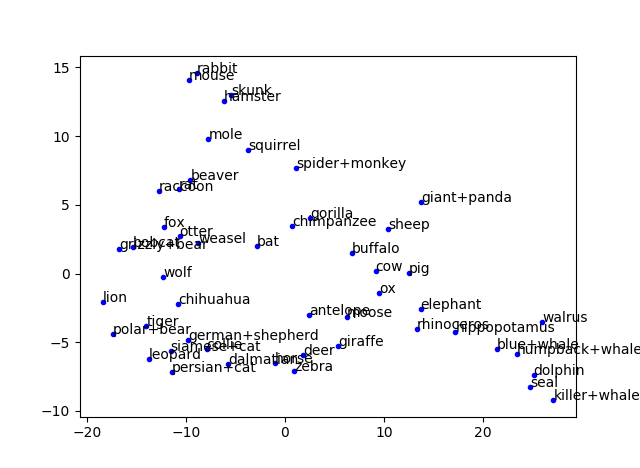
\includegraphics[width=50em,height=8.5cm]{q2_1.png}
    \caption{Question 2.1 ISOMAP}
    \label{fig:q2_1}
\end{figure}

Code:
\begin{verbatim}

function ISOMAP(X)
    k =3
    (n,d) = size(X)

    # Compute all distances
    D = distancesSquared(X,X)
    D = sqrt.(abs.(D))

    E = ones(n,n).*Inf

    for i in 1:n
        A = sortperm(D[i,:])
        for j in 2:k+1
          
          E[i,A[j]] =D[i,A[j]]
          E[A[j],i] =D[A[j],i]     
        end 
    end

    D = zeros(n,n)
    for i in 1:n
        for j in 1:n
         D[i,j] = dijkstra(E,i,j)
        end
    end

    # Initialize low-dimensional representation with PCA
    model = PCA(X,2)
    Z = model.compress(X)
    

    funObj(z) = stress(z,D)

    Z[:] = findMin(funObj,Z[:])

    return Z
end

\end{verbatim}



\subsection{ISOMAP with Disconnected Graph}

An issue with measuring distances on graphs is that the graph may not be connected. For example, if you run your ISOMAP code with $2$-nearest neighbours then some of the distances are infinite. One heuristic to address this is to set these infinite distances to the maximum distance in the graph (i.e., the maximum geodesic distance between any two points that are connected), which will encourage non-connected points to be far apart. Modify your ISOMAP function to implement this heuristic. \blu{Hand in your code and the plot of the result when using the $2$-nearest neighbours}.

\begin{figure}[h!]
    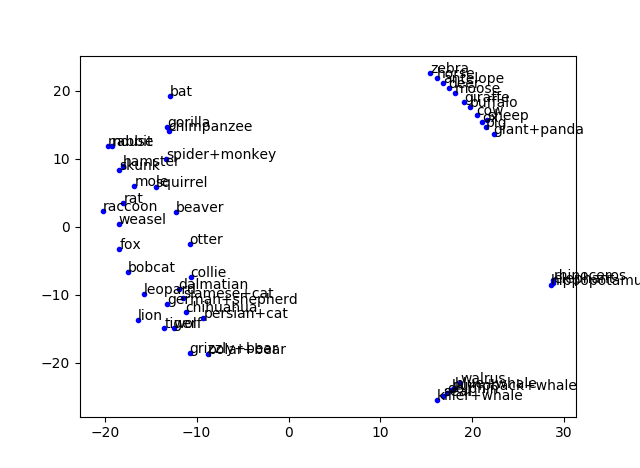
\includegraphics[width=50em,height=8.5cm]{q2_2.png}
    \caption{Question 2.2 ISOMAP with Disconnected Graph}
    \label{fig:q2_2}
\end{figure}

Code:
\begin{verbatim}

function ISOMAPdisconnectedGraph(X)
    k =2
    (n,d) = size(X)

    # Compute all distances
    D = distancesSquared(X,X)
    D = sqrt.(abs.(D))

    E = ones(n,n).*Inf

    for i in 1:n
        A = sortperm(D[i,:])
        for j in 2:k+1
          
          E[i,A[j]] =D[i,A[j]]
          E[A[j],i] =D[A[j],i]     
        end 
    end

    D = zeros(n,n)
    max = -Inf
    for i in 1:n
        for j in 1:n
         D[i,j] = dijkstra(E,i,j)
         if(D[i,j]!=Inf && D[i,j] > max)
            max =  D[i,j]
         end
        end
    end


    for i in 1:n
        for j in 1:n
             if(D[i,j]==Inf )
             D[i,j] = max
         end
        end
    end


    # Initialize low-dimensional representation with PCA
    model = PCA(X,2)
    Z = model.compress(X)
    

    funObj(z) = stress(z,D)

    Z[:] = findMin(funObj,Z[:])

    return Z
end

\end{verbatim}


\section{Neural Networks}

Various changes were made using combinations of the following items:
\items{
\item increasing $nHidden$ up to 150
\item increasing and decreasing the stochastic gradient step-size
\item increasing the number of stochastic iterations
\item adding momentum
\item adding L2 regularizer with various values for $\lambda$
\item using different activation functions, such as sigmoid, quadratic, $tanh + tanh^2$, composite of $tanh$ and quadratic
}

(standardization wasn't tried because the data we are graphing is 2D - i.e. we're only fitting 1 feature)

In the end, the best fit we found had the following parameters and added steps:
\items{
    \item $nHidden = 100$: deep neural network
    \item L2 regularizer with $\lambda = 0.01$: to reduce overfitting since we have so many layers
    \item momentum: to improve optimization using stochastic gradient
    \item dynamic step size, going from $1e-4$ to $1e-7$: deep networks are sensitive to step-size, so the idea was to improve the performance of stochastic gradient by decreasing the step-size. We used decreasing step-sizes instead of using a constant small step-size to reduce runtime and the number of iterations required
    \item 50000 iterations: stochastic gradient with smaller step-sizes requires more iterations to reach optimal region
}

\begin{figure}[h!]
    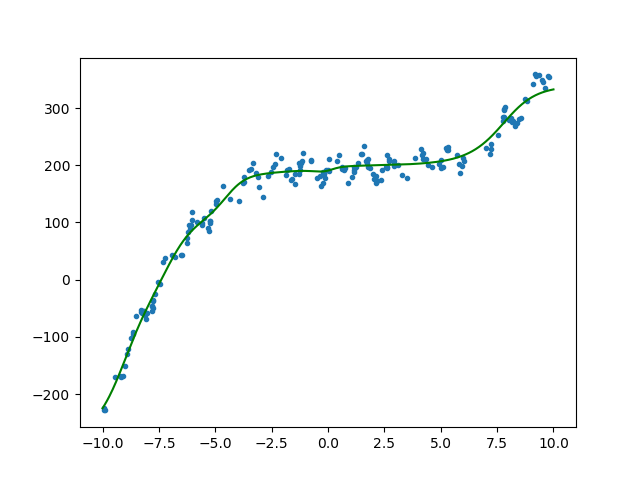
\includegraphics[width=28em]{a5_q3.png}
    \caption{Improved Neural Network Result}
    \label{fig:q3}
\end{figure}

\section{Very-Short Answer Questions}


\enum{
\item NMF is non-convex and can be minimized using projected gradient, where we run gradient descent on the loss function but set any negative values we get from gradient descent to zero.
\item A standard collaborative filtering model is trained, unsupervised, to minimize categorizing/clustering errors and is never trained to optimize the weights for prediction with supervised learning.
\item No. Both MDS and PCA can be viewed as some sort of compression algorithms, so there is always data loss, unless the data points in 3D all lie on the same 2D plane, but that's not guaranteed.
\item Euclidean distance is the length of the straight line drawn between two points, whereas geodesic distance is the length of the curve drawn between two points on a manifold. (i.e. Euclidean $\leq$ geodesic)
\item It results in a smooth loss that can be optimized with gradient descent and ensures the output of the perceptron is between 0 and 1 regardless of the domain of the input, so it can be used to represent probabilities
\item A deeper neural network likely has a higher test error but lower train error, while a neural network less deep likely has a high train error but lower test error.
\item 1) adding L2-regularizers for each layer of $W$ and optimizing the $\lambda$ of each regularizer, 2) early stopping (stops optimzation if validation error starts increasing), 3) dropout (setting some $x_i$ and $z_i$ in each layer to 0)
\item  Larger width results in smaller train error but larger test error, whereas smaller width results in larger train error but smaller test error.
}

\end{document}
